% ORS 2027 Annual Meeting abstract: the DRD-3 three-chamber dynamic release device.
% Compile with tectonic (XeTeX engine):  tectonic ors-2027-abstract.tex
% Format follows ORS rules: Times New Roman 8pt, 0.75in margins, single page,
% sections Introduction/Methods/Results/Discussion/Significance + References, up to 3 figures/tables.
%
% OPEN ITEMS for Filippo to confirm before submission:
%   1. Author list and order (defaulted to the published-DRD lab seniors; confirm with Dr. Asik).
%   2. The \tbd{...} placeholders mark experimental numbers that are still pending; drop in real
%      values as Phase 0/1/2 validation completes. Search the file for "\tbd".
%   3. Funding lines in Acknowledgements.

\documentclass[8pt]{extarticle}

\usepackage[letterpaper,margin=0.75in]{geometry}
\usepackage{fontspec}
\usepackage{xcolor}
\usepackage{multicol}
\usepackage{enumitem}
\usepackage{tikz}
\usetikzlibrary{patterns,arrows.meta}
\usepackage{graphicx}
\graphicspath{{figures/}}
\usepackage{microtype}

% --- literal Times New Roman, matching the ORS template ---
% Font files are bundled in fonts/ so this compiles unchanged both locally
% (tectonic) and on Overleaf (XeLaTeX) without relying on system fonts.
\setmainfont{Times New Roman}[
  Path = fonts/ ,
  Extension = .ttf ,
  UprightFont = * ,
  BoldFont = * Bold ,
  ItalicFont = * Italic ,
  BoldItalicFont = * Bold Italic ,
]

% --- brand palette carried over from the deck ---
\definecolor{tealc}{HTML}{16767B}   % drug hub / joint
\definecolor{perf}{HTML}{2D6CB0}     % perfusion
\definecolor{coral}{HTML}{C0552E}    % bacteria
\definecolor{tbdcol}{HTML}{B23A00}   % pending-value marker

% pending experimental values, easy to spot and to grep
\newcommand{\tbd}[1]{{\color{tbdcol}\textbf{[#1]}}}

% run-in section heading, ORS style
\newcommand{\osec}[1]{\par\vspace{1.5pt}\noindent{\bfseries\color{tealc}#1.}\hspace{0.6em}\ignorespaces}

\setlength{\parindent}{0pt}
\setlength{\columnsep}{16pt}
\setlength{\columnseprule}{0.3pt}
\renewcommand{\columnseprulecolor}{\color{tealc!55}}
\emergencystretch=1em
\pagestyle{empty}

\begin{document}

% ============================ TITLE BLOCK ============================
\begin{center}
  {\fontsize{13}{15}\selectfont\bfseries
   A Three-Chamber Dynamic Release Device for Simultaneous Drug-Release Kinetics
   and \textit{In Situ} Infection Challenge of Drug-Eluting Ultra-High-Molecular-Weight
   Polyethylene (UHMWPE) Joint Implants\par}
  \vspace{5pt}
  {\fontsize{10}{12}\selectfont
   Filippo Fonseca\textsuperscript{1,2}, Mehmet D. Aşık\textsuperscript{2},
   Ebru Oral\textsuperscript{2}, Orhun K. Muratoglu\textsuperscript{2}\par}
  \vspace{3pt}
  {\footnotesize\itshape
   \textsuperscript{1}Yale University, New Haven, CT, USA.\quad
   \textsuperscript{2}Harris Orthopaedics Laboratory, Massachusetts General Hospital and
   Harvard Medical School, Boston, MA, USA.\par}
  \vspace{2pt}
  {\footnotesize Presenting author: Filippo Fonseca \textnormal{(filippo.fonseca@yale.edu)}\par}
\end{center}

\vspace{2pt}
{\color{tealc!60}\hrule height 0.6pt}
\vspace{4pt}

% ============================ FIGURE 1 (full width) ============================
\begin{center}
\resizebox{0.63\textwidth}{!}{%
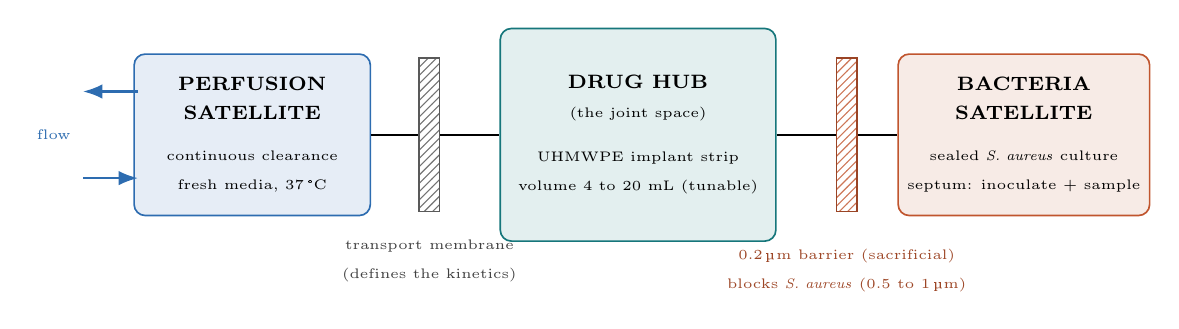
\begin{tikzpicture}[>=Latex, line width=0.6pt]
  % --- three chambers ---
  \node[draw=perf, fill=perf!12, rounded corners, minimum width=3.0cm, minimum height=2.05cm,
        align=center] (perf) at (1.9,0)
        {\scriptsize\textbf{PERFUSION}\\[-1.5pt]\scriptsize\textbf{SATELLITE}\\[3pt]
         \tiny continuous clearance\\[-1.5pt]\tiny fresh media, 37\,°C};
  \node[draw=tealc, fill=tealc!12, rounded corners, minimum width=3.5cm, minimum height=2.7cm,
        align=center] (hub) at (6.8,0)
        {\scriptsize\textbf{DRUG HUB}\\[-1.5pt]\tiny (the joint space)\\[4pt]
         \tiny UHMWPE implant strip\\[-1.5pt]\tiny volume 4 to 20 mL (tunable)};
  \node[draw=coral, fill=coral!12, rounded corners, minimum width=3.0cm, minimum height=2.05cm,
        align=center] (bact) at (11.7,0)
        {\scriptsize\textbf{BACTERIA}\\[-1.5pt]\scriptsize\textbf{SATELLITE}\\[3pt]
         \tiny sealed \emph{S. aureus} culture\\[-1.5pt]\tiny septum: inoculate + sample};
  % --- membranes in the two gaps ---
  \node[draw=black!65, minimum width=0.26cm, minimum height=1.95cm,
        pattern=north east lines, pattern color=black!55] (mt) at (4.15,0) {};
  \node[draw=coral!80!black, minimum width=0.26cm, minimum height=1.95cm,
        pattern=north east lines, pattern color=coral!80] (mb) at (9.45,0) {};
  \draw (perf.east) -- (mt.west); \draw (mt.east) -- (hub.west);
  \draw (hub.east) -- (mb.west);  \draw (mb.east) -- (bact.west);
  % --- membrane labels ---
  \node[align=center, text=black!75] at (4.15,-1.6)
        {\tiny transport membrane\\[-1.5pt]\tiny (defines the kinetics)};
  \node[align=center, text=coral!82!black] at (9.45,-1.72)
        {\tiny 0.2\,µm barrier (sacrificial)\\[-1.5pt]\tiny blocks \emph{S. aureus} (0.5 to 1\,µm)};
  % --- perfusion flow arrows ---
  \draw[->, perf, line width=0.9pt] (0.45,0.55) -- (-0.25,0.55);
  \draw[<-, perf, line width=0.9pt] (0.45,-0.55) -- (-0.25,-0.55);
  \node[perf, align=center] at (-0.62,0) {\tiny flow};
\end{tikzpicture}}
\\[-1pt]
{\footnotesize\bfseries\color{tealc}(A)} {\footnotesize\itshape radial three-chamber concept}

\vspace{1pt}

% --- row of three CAD views (B, C, D) ---
\setlength{\tabcolsep}{6pt}
\begin{tabular}{@{}ccc@{}}
  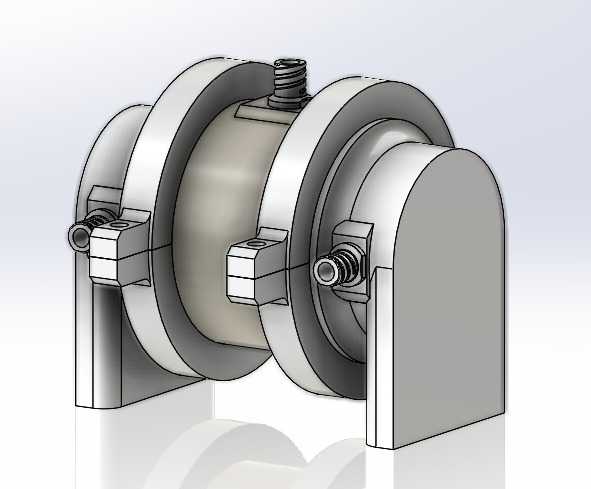
\includegraphics[height=1.62cm]{hero_full_assembly.jpg} &
  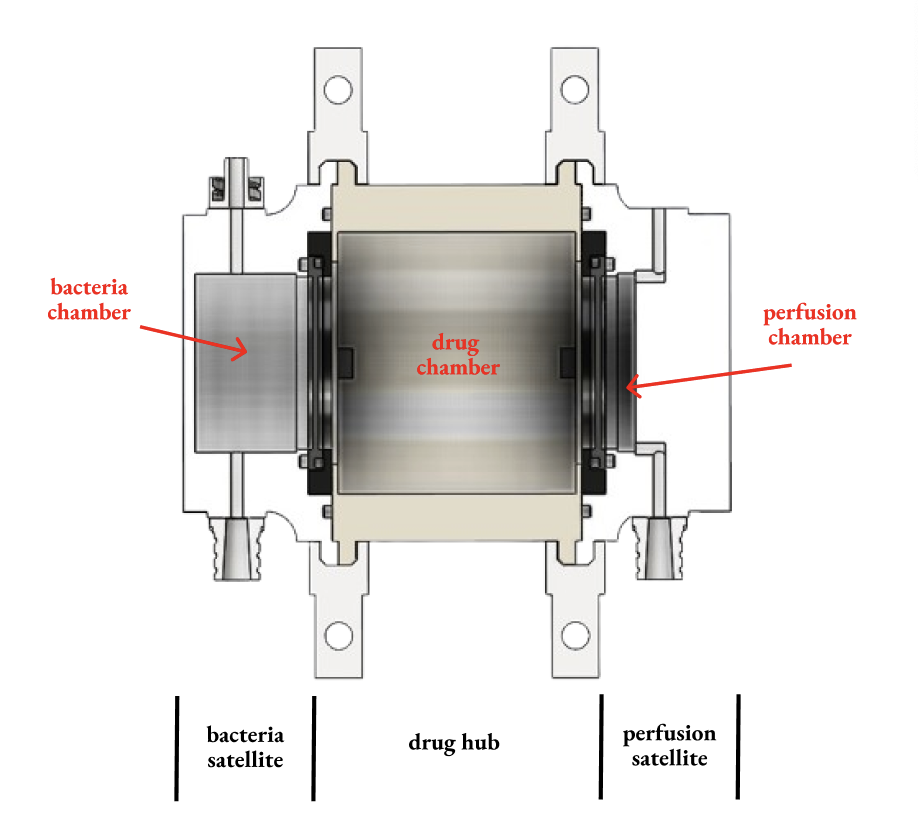
\includegraphics[height=1.62cm]{topdown_sectioned.jpg} &
  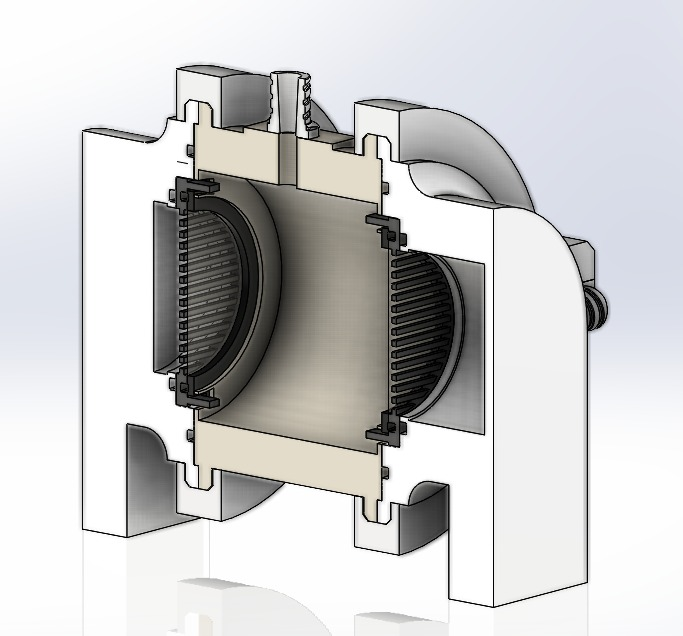
\includegraphics[height=1.62cm]{section_iso_membranes.jpg} \\[0pt]
  {\footnotesize\bfseries\color{tealc}(B)} {\footnotesize as-modeled assembly} &
  {\footnotesize\bfseries\color{tealc}(C)} {\footnotesize sectioned chambers} &
  {\footnotesize\bfseries\color{tealc}(D)} {\footnotesize opposite-face membranes} \\
\end{tabular}
\end{center}
\vspace{1pt}
{\footnotesize\textbf{Figure 1.} The DRD-3 three-chamber device.
\textbf{(A)} Radial schematic: a central drug hub (joint space, holding the UHMWPE strip) is flanked on
opposite faces by a perfusion satellite and a sealed bacteria satellite; placing the two membranes on
opposite faces rather than in series keeps biofilm on the sacrificial 0.2\,µm barrier from reaching the
transport membrane that sets the kinetics. \textbf{(B)} As-modeled assembly with the C-ring wrappers
that load each joint. \textbf{(C)} Top-down section through the three chambers. \textbf{(D)} Isometric
cut showing the two opposite-face membranes in modular cartridges. Sealing uses three identical O-ring
pairs (2.0\,mm cord, 25\% compression).\par}
\vspace{2pt}

% ============================ BODY (two columns) ============================
\begin{multicols}{2}
\small
\linespread{0.955}\selectfont

\osec{Introduction}
Periprosthetic joint infection (PJI) remains one of the most serious complications after total joint arthroplasty. An otherwise successful reconstruction can be converted into a prolonged course of revision surgery and antibiotic treatment, leading to impaired function and increased patient morbidity.\textsuperscript{1,2} Although systemic antibiotics are routinely used in PJI treatment, achieving sustained therapeutic concentrations inside the joint is difficult because intraarticular drug availability is limited by local transport barriers, synovial fluid interactions, and the need to avoid toxic serum concentrations.\textsuperscript{1,3} Local antibiotic delivery from drug-eluting implants is therefore attractive because it can concentrate drug at the site of infection while reducing systemic exposure.

Ultra-high-molecular-weight polyethylene (UHMWPE) is the material of choice for load-bearing total joint implants, and antibiotic-eluting UHMWPE is being developed as a functional spacer or implant material for PJI treatment.\textsuperscript{1,2} Translation of these materials requires in-vitro models that capture the release, transport, and clearance conditions governing drug concentration inside the joint. The Dynamic Release Device (DRD) was recently developed to address this need by combining a drug chamber representing the joint space, a diffusion membrane representing synovial transport, and a perfused chamber representing clearance.\textsuperscript{3} However, the DRD evaluates drug transport without a live infection challenge, as the current design would mean adding bacteria directly to the drug chamber; this would allow biofilm to foul the transport membrane, thus altering the permeability that defines the measured release kinetics. In this study, we designed a three-chamber DRD-3 to preserve the DRD transport measurement while adding a physically isolated \emph{Staphylococcus aureus} challenge in the same experiment, furthering our understanding of intrarticular dynamics by simualting the infection-based scenario where a drug-eluding antiobiotic would be most useful.

\osec{Methods}
We designed a clean-sheet, three-chamber device (the DRD-3) in CAD (Fig.~1A; assembly in Fig.~1B). A central drug hub
represents the joint space, holds the UHMWPE implant strip, and targets a tunable fluid volume of
4 to 20\,mL spanning healthy to infected knee synovial volumes. The hub is flanked on opposite faces
by two satellites: a perfusion satellite providing continuous fresh-media clearance (the validated
transport physics, preserved) and a bacteria satellite housing a sealed culture (Fig.~1C). Because the two
membranes sit on opposite faces of the hub rather than stacked in series (Fig.~1D), neither membrane is exposed
to the other's fouling. Each membrane is sealed off-device inside a modular lid-and-base cartridge; a
single tapered tooth (tapering from 2.0 to 1.0\,mm) both captures the membrane sandwich and retains
the finished cartridge in its satellite, and parallel protective bars shield the membrane from the
UHMWPE strip without restricting diffusion. Every sealing interface uses one identical static O-ring
specification (2.0\,mm cord, 1.5\,mm gland, 0.5\,mm stand-proud giving 25\% compression), so the
entire two-membrane device seals on three identical O-ring pairs. Each satellite is drawn to the hub
by a two-piece C-ring wrapper whose U-channel applies uniform radial load around the joint with one
bolt per side, replacing point-loaded flange bolts. Bacterial isolation is enforced by a sacrificial
0.2\,µm microfilter on the bacteria-facing membrane that passes drug freely but physically blocks
\emph{S. aureus} (0.5 to 1\,µm) from migrating toward the transport membrane; the culture is accessed
through a self-sealing septum for inoculation and colony-forming-unit (CFU) sampling without breaching
sterility. Structural parts are stereolithography (SLA) resins (Accura-60-class chassis; Somos 9120
for the compliant inner cartridge parts) with medical-grade silicone/EPDM (USP Class VI) O-rings. A
three-phase validation protocol is defined: Phase~0, a dye-perfusion leak test at 64\,mL/h for 24\,h
(acceptance below 2\% volume loss per 24\,h); Phase~1, reproduction of the published release kinetics
across flow rate (2 to 64\,mL/h), temperature (room temperature versus 37\,°C), and membrane
thickness; and Phase~2, introduction of \emph{S. aureus} in the bacteria satellite with CFU sampling
over 24\,h to confirm zero bacterial migration to the perfusion side. As a non-clinical benchtop
instrument, this work involves no human or animal subjects, and sex as a biological variable is not
applicable at this stage.

\osec{Results}
A complete three-chamber DRD-3 was realized in CAD. The design consolidates all sealing to three
identical O-ring pairs and a single tapered-tooth feature that performs both membrane capture and
cartridge retention, and it replaces the earlier multi-bolt, point-loaded clamp with one continuous
C-ring wrapper per satellite (four wrappers, one bolt per side) that distributes radial load uniformly
around each joint. The 0.2\,µm isolation barrier is sized well below the \emph{S. aureus} cell
diameter, and the drug hub is parameterized so hub depth can be tuned to a target volume. The
as-modeled internal volume is being extracted from CAD to confirm it lands in the 4 to 20\,mL window
\tbd{measured volume, mL}. Experimental validation is in progress: Phase~0 leak loss
\tbd{value \% / 24\,h}; Phase~1 agreement of DRD-3 half-life trends with the published baseline
\tbd{result}; Phase~2 bacterial count on the perfusion side \tbd{CFU; expected 0}.

\osec{Discussion}
The defining feature of the DRD-3 is the radial, opposite-face, two-membrane architecture, which
decouples the infection challenge from the transport measurement. Biofilm is permitted, and can
optionally be imaged through a swappable borosilicate window, on the sacrificial barrier, while the
kinetics-defining membrane stays clean. The modular design targets the reproducibility and assembly
failure modes of press-fit SLA stacks: the membrane is sealed as a bench-built module, the seal is an
elastomer rather than a flexing printed feature, and the wrapper clamp removes press-fit interfaces
from the load path. Limitations are that the as-modeled internal volume is not yet verified against
the 4 to 20\,mL target; the experimental validation (leak integrity, kinetics reproduction, and
isolation) is ongoing; SLA parts must be fully post-cured and washed before live-culture runs to avoid
residual-monomer antimicrobial bias; and the bacteria and perfusion chamber volumes are currently
asymmetric, which is under review. The mapping to anatomy is also deliberately partial: the drug hub
represents the intraarticular space and the perfusion satellite the joint's clearance pathway, but the
isolated bacterial compartment is an engineering abstraction rather than an anatomical analog (in vivo
the infection resides within the joint space itself), adopted so that biofilm cannot foul the
transport membrane that defines the kinetics. Within the framework of our objective, the device is built so that,
once it reproduces the published transport baseline, it can add a live antimicrobial-efficacy readout
without compromising that measurement.

\osec{Significance}
This platform would allow drug-eluting UHMWPE bearing materials to be screened for both intraarticular
release kinetics and live antimicrobial efficacy on a single benchtop, directly supporting the
development of local-delivery strategies against periprosthetic joint infection.

\osec{Acknowledgements}
The authors thank the Harris Orthopaedics Laboratory. \tbd{funding sources}

\osec{References}
\footnotesize
\begin{enumerate}[leftmargin=1.2em,nosep,label=\arabic*.]
\item Aşık MD, Zhao T, Fan Y, Ferreira M, Yang L, Inverardi N, Sekar A, Fujino K,
Ben Malick F, Wannomae KK, Oral E, Muratoglu OK. Advancing joint infection
treatment: long-term animal implantation of submicron gentamicin-loaded UHMWPE.
\textit{J Biomed Mater Res B Appl Biomater}. 2025;113:e35673.

\item Aşık MD, Walsh-Rock E, Inverardi N, Nepple C, Zhao T, Sekar A,
Dutta Kannambadi D, Ferreira M, Wannomae KK, Oral E, Muratoglu OK.
Enhanced antibiotic release and mechanical strength in UHMWPE antibiotic blends:
the role of submicron gentamicin sulfate particles.
\textit{J Bone Joint Surg Am}. 2025;107:586--593.

\item Aşık MD, Reyhanli A, Serafim MF, Inverardi N, Muratoglu OK, Oral E.
A dynamic device to simulate intraarticular drug-release kinetics.
\textit{Int J Pharm}. 2026;695:126738.
\end{enumerate}

\end{multicols}
\end{document}

